\documentclass{beamer}

\mode<presentation> {
  \usetheme{PaloAlto}
}

%%
\makeatletter
\setbeamertemplate{subsubsection in sidebar}{\vspace*{-\baselineskip}}
\setbeamertemplate{subsubsection in sidebar shaded}{\vspace*{-\baselineskip}}
\makeatother
%%

%%
\setbeamertemplate{theorems}[numbered]
%%

\definecolor{Garnet}{RGB}{130,0,20}
\usecolortheme[named=Garnet]{structure}

\logo{
\includegraphics[width=1.5cm]{../../sharedImgs/USClogo.png}}

%\setbeamercolor{title}{fg=red!60!black,bg=white!50!black}
%\usecolortheme{beaver}
%\usecolortheme{crane}
\usefonttheme{structuresmallcapsserif}
\usefonttheme[onlysmall]{structurebold}

\usepackage{multicol}
\usepackage{graphicx}
\usepackage{mathtools}
\usepackage{latexsym}
\usepackage{amsfonts}
\usepackage[only,ninrm,elvrm,twlrm,sixrm,egtrm,tenrm]{rawfonts}
\usepackage{indentfirst}
\usepackage[noend]{algorithmic}
\usepackage{algorithm}
\usepackage{enumerate}
\usepackage{graphicx,psfrag}
\usepackage{epsfig}
%\usepackage[pdflatex]{graphicx}
%\usepackage{epstopdf}
\usepackage{ulem}
\usepackage{animate} %need the animate.sty file
\usepackage{tikz}
\usetikzlibrary{fit,shapes,calc}
\usepackage{pgfplots}
\usepackage{amsmath,amsthm,amssymb,amsfonts,enumerate,mymath,mathtools,tikz-cd,mathrsfs}

\newtheorem{thm}{Theorem}
\newtheorem{lem}{Lemma}
\newtheorem{prop}{Proposition}
\theoremstyle{definition}
\newtheorem{defn}{Definition}
\newtheorem{rmk}{Remark}

\newcommand{\A}{\mathscr{A}}
\renewcommand{\C}{\mathscr{C}}

\newcommand*{\defeq}{\mathrel{\vcenter{\baselineskip0.5ex \lineskiplimit0pt
                     \hbox{\scriptsize.}\hbox{\scriptsize.}}}%
                     =}
\DeclarePairedDelimiter\ceil{\lceil}{\rceil}
\DeclarePairedDelimiter\floor{\lfloor}{\rfloor}

\input epsf



\usepackage[english]{babel}
% or whatever

\usepackage[latin1]{inputenc}
% or whatever

\usepackage{times}
\usepackage[T1]{fontenc}
% Or whatever. Note that the encoding and the font should match. If T1
% does not look nice, try deleting the line with the fontenc.

\title % (optional, use only with long paper titles)
    {Graph Transformations}

\author[Farman]
{Blake Farman~\inst{1}}

\institute[USC]{
\inst{1}
University of South Carolina, Columbia, SC USA}
%\inst{2}
%East Carolina University, Greenville, NC USA\\
%\inst{3}
%University of Johannesburg, Auckland Park, South Africa}

\date[January 17, 2017]
{Math 122: Calculus for Business Administration and Social Sciences}

%\subject{Irredundant and Mixed Ramsey Numbers}
\setbeamercolor{alerted text}{fg=red!60!black}
\setbeamercolor{block title}{bg=white!50!black,fg=red!60!black}

\begin{document}

\begin{frame}
  \titlepage
\end{frame}

\begin{frame}
  \frametitle{Outline}
  \tableofcontents[pausesections]
\end{frame}

\section{1.8: New Functions from Old}

\subsection{Function Composition}
\begin{frame}{Function Composition}
  \begin{defn}
    Given a function $f$ and a function $g$ such that the range of $f$ is contained in the domain of $g$ we can define the composition
    $$g \circ f(x) = g\left(f\left(x\right)\right).$$
  \end{defn}
  \onslide<2->{
  \begin{rmk}
    We require that the range of $f$ is contained in the domain of $g$ so that the composition makes sense.
    \onslide<3->{That is, we don't want $f(x)$ to be a point for which $g$ is undefined.}
  \end{rmk}
  }
\end{frame}

\begin{frame}{Example}
  Let
  \begin{itemize}
  \item<1->
    $f(x) = x + 1$, and
  \item<2->
    $g(x) = x^2$.
  \end{itemize}
  \onslide<3->{Both have domain and range $\R$, so we can compose in either order}.
  \onslide<4->{
    $$g \circ f(x) = g\left(f\left(x\right)\right) \onslide<5->{= g(x + 1)} \onslide<6->{= (x + 1)^2} \onslide<7->{= x^2 + 2x + 1.}$$}
  \onslide<8->{and
    $$f \circ g(x) = f\left(g\left(x\right)\right) \onslide<9->{= f(x^2)} \onslide<10->{= x^2 + 1.}$$}
\end{frame}


\begin{frame}{Example}
  Let 
  \begin{itemize}
    \item<1->
      $f(x) = \frac{1}{x}$, and
    \item<2->
      $g(x) = x - 1$.
  \end{itemize}
  \onslide<3->{The domain and range of $g$ are both $\R$}.
  \onslide<4->{The domain and range of $f$ are both
    $$\left\{x \in \R \;\middle\vert\; x \neq 0 \right\}.$$}
  \onslide<5->{If we restrict $g(x)$ to the domain 
    $$\left\{x \in \R \;\middle\vert\; x \neq 1\right\}$$
    then $g(x) \neq 0$.}
  \onslide<6->{Hence
    $$f \circ g(x) = \frac{1}{x - 1}.$$}
\end{frame}

\subsection{Scaling}

\begin{frame}{Vertical Scaling}
  \onslide<1->{Let $f(x)$ be a function and let $0 < a$ be a real number.}
  \onslide<2->{The graph of $af(x)$ is
    \begin{itemize}
      \item<3->a {\it vertical stretching} of the graph of $f(x)$ if $1 < a$
      \item<4->a {\it vertical shrinking} of the graph of $f(x)$ if $a < 1$.
    \end{itemize}
  }
\end{frame}

\begin{frame}{Examples}
  \begin{center}
    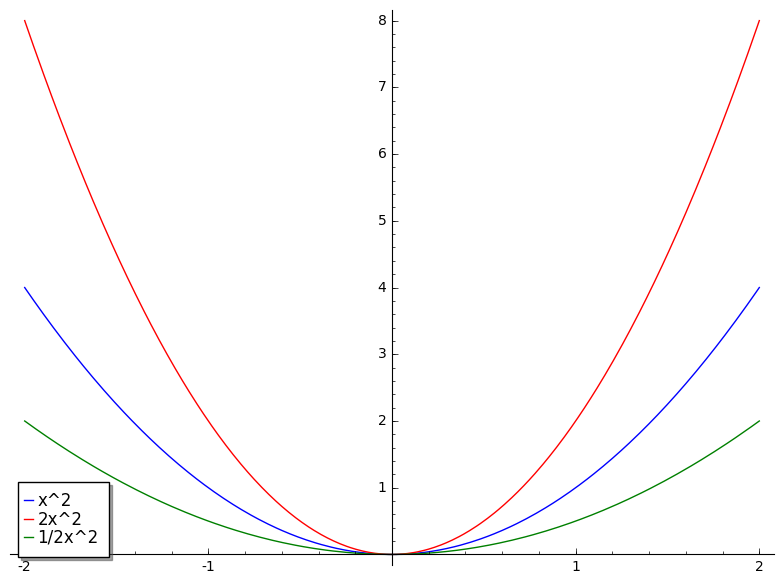
\includegraphics[scale=0.5]{imgs/scaling.png}
  \end{center}
\end{frame}
\subsection{Rigid Transformations}
\begin{frame}{Reflection}
  The graph of $-f(x)$ is a reflection of $f(x)$ across the $x$-axis.
  \begin{center}
    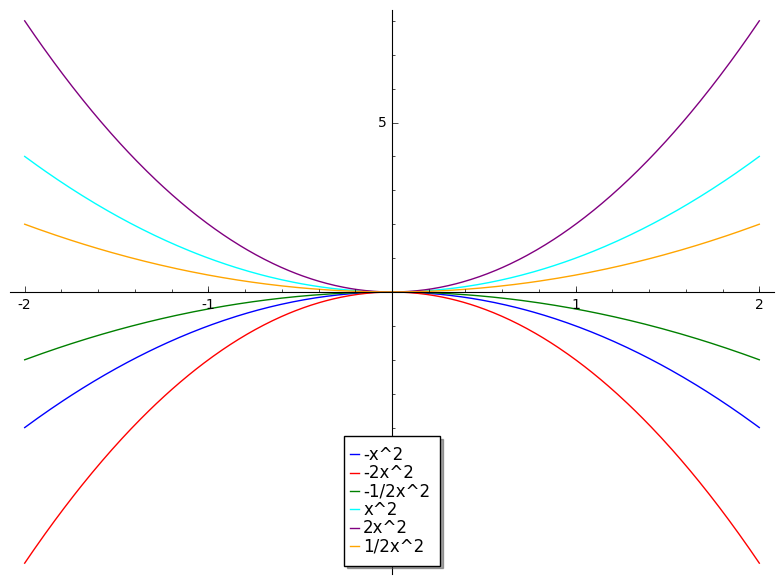
\includegraphics[scale=0.4]{imgs/reflections.png}
  \end{center}
\end{frame}

\begin{frame}{Vertical Shifting}
  Let $f(x)$ be a function.
  \onslide<2->{Let $0 < a$ be a real number.}
  \begin{itemize}
    \item<3->
      The graph of $f(x) + a$ is the graph of $f(x)$ shifted up $a$ units.
    \item
      <4->
      The graph of $f(x) - a$ is the graph of $f(x)$ shifted down $a$ units.
  \end{itemize}
\end{frame}

\begin{frame}{Examples}
  \begin{center}
    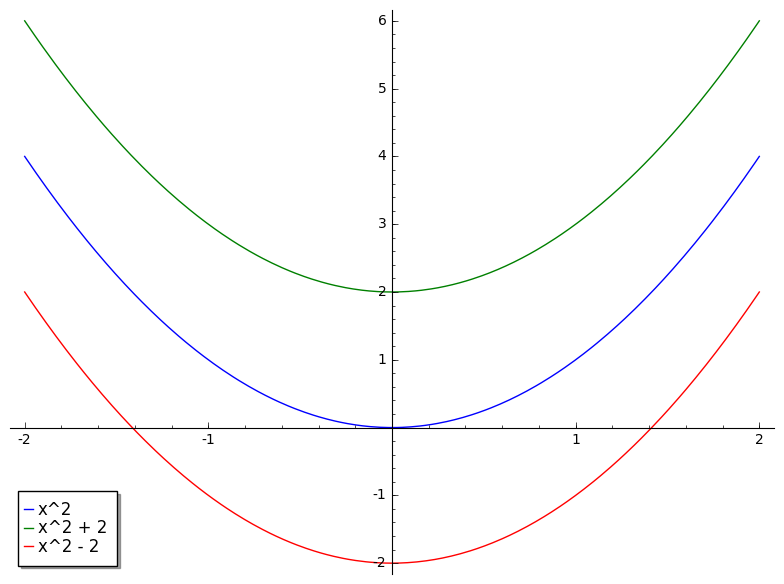
\includegraphics[scale=0.4]{imgs/vertShift.png}
  \end{center}
\end{frame}

\begin{frame}{Horizontal Shifting}
  Let $f(x)$ be a function.
  \onslide<2->{Let $0 < a$ be a real number.}
  \begin{itemize}
    \item<3->
      The graph of $f(x - a)$ is a horizontal shift of $f(x)$ by $a$ units to the right.
    \item<4->
      The graph of $f(x + a)$ is a horizontal shift of $f(x)$ by $a$ units to the left.
  \end{itemize}
\end{frame}

\begin{frame}{Examples}
  \begin{center}
    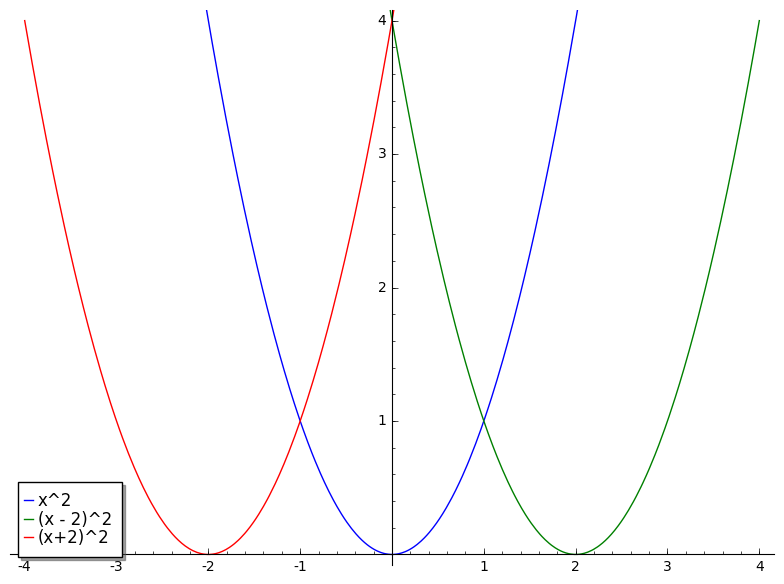
\includegraphics[scale=0.5]{imgs/horizShifts.png}
  \end{center}
\end{frame}
\end{document}
